\documentclass[a4paper,10pt]{article}

\usepackage[T1]{fontenc}
\usepackage[utf8]{inputenc}
\usepackage{textcomp}
\usepackage{fontspec}
\usepackage{graphicx}
\usepackage{xcolor, colortbl}
\usepackage{caption}
\usepackage{listings}
\usepackage{wrapfig} 
\usepackage{tabu} % For coloring single row of table
\usepackage{scrextend}

\usepackage{tgheros}

\usepackage{amsmath,amssymb,amsthm,textcomp}
\usepackage{enumerate}
\usepackage{multicol}
\usepackage{tikz}

\usepackage{geometry}
\usepackage{trace}
\usepackage{tcolorbox}
\usepackage{tabularx}
\usepackage{accsupp}% http://ctan.org/pkg/accsupp
\usepackage{enumitem}

%% For using numbers at every level of enumerated list
\newlist{legal}{enumerate}{10}
\setlist[legal]{label*=\arabic*.}

\tcbuselibrary{listings,skins} % For lstlisting

\geometry{total={210mm,297mm},
left=25mm,right=25mm,%
bindingoffset=0mm, top=20mm,bottom=20mm}


% For coloring single row in table
\def\zapcolorreset{\let\reset@color\relax\ignorespaces}
\def\colorrows#1{\noalign{\aftergroup\zapcolorreset#1}\ignorespaces}

\newcommand{\linia}{\rule{\linewidth}{0.5pt}}
\newcommand{\ano}{\text{2}}

% custom theorems if needed
\newtheoremstyle{mytheor}
    {1ex}{1ex}{\normalfont}{0pt}{\scshape}{.}{1ex}
    {{\thmname{#1 }}{\thmnumber{#2}}{\thmnote{ (#3)}}}

\theoremstyle{mytheor}
\newtheorem{defi}{Definition}

%%% Declare title %%%%%%%%%%%%%%%%%%%%%%%%%%%%%%%%%%%%%%%%%%%%%%%% 
\newcommand{\antitle}{\text{Verilog Modelling Techniques}}
% my own titles
\makeatletter
\renewcommand{\maketitle}{
\begin{center}
\vspace{2ex}
{\huge \textsc{{{\large}Assignment - \ano}\vspace{0.1cm} \break \antitle}}
\vspace{1ex}
\\
%%%%%%%%%%%%%%%%%%%%%%%%%%%%%%%%%%%%%%%%%%%%%%%%%%%%%%%%%%%%%%%%%%

Department of Electronics and Communication Engineering \\
Indian Institute of Technology, Roorkee
\linia\\
ECN 104 \hfill Digital Logic Design
\vspace{4ex}
\end{center}
}
\makeatother
%%%

% custom footers and headers
\usepackage{fancyhdr}
\pagestyle{fancy}
\lhead{}
\chead{}
\rhead{}
\lfoot{Assignment \ano\ - \antitle}
\cfoot{}
\rfoot{Page \thepage}
\renewcommand{\headrulewidth}{0pt}
\renewcommand{\footrulewidth}{0pt}
%

\definecolor{vgreen}{RGB}{104,180,104}
\definecolor{vblue}{RGB}{49,49,255}
\definecolor{vorange}{RGB}{255,143,102}

\makeatletter
\newcommand*\@lbracket{[}
\newcommand*\@rbracket{]}
\newcommand*\@colon{:}
\newcommand*\colorIndex{%
    \edef\@temp{\the\lst@token}%
    \ifx\@temp\@lbracket \color{black}%
    \else\ifx\@temp\@rbracket \color{black}%
    \else\ifx\@temp\@colon \color{black}%
    \else \color{vorange}%
    \fi\fi\fi
}
\makeatother

\definecolor{codebg}{RGB}{250,250,240} 
\definecolor{greatblue}{RGB}{91,155,215}  
\definecolor{infocolor}{RGB}{102, 51, 153} 

% Set up caption and labels for lstlistings
\DeclareCaptionFont{white}{\color{white}}
\DeclareCaptionFormat{listing}{\colorbox{greatblue}{\parbox{\textwidth}{\hspace{1cm}#1#2#3}}}
\captionsetup[lstlisting]{format=listing,labelfont=white,textfont=white}

\renewcommand{\thelstnumber}{% Line number printing mechanism
  \protect\BeginAccSupp{ActualText={}}\arabic{lstnumber}\protect\EndAccSupp{}%
}

\renewcommand\familydefault{\sfdefault} 
\usepackage[T1]{fontenc}

% -----------------------------------------------------------
% Comment the following lines if Source Code Pro font is
% not available

\newfontfamily\listingsfont[Scale=0.8]{Source Code Pro} 
\newfontfamily\listingsfontinline[Scale=0.8]{Source Code Pro}
% -----------------------------------------------------------

\def\backtick{\char18} 
\lstdefinestyle{verilog-style}
{
    %columns=fullflexible, 
    language=Verilog,
    basicstyle=\listingsfont,
    keywordstyle=\color{vblue},
    identifierstyle=\color{black},
    commentstyle=\color{vgreen},
    numbers=left, 
    numberstyle=\color{gray},  
    numbersep=10pt,
    moredelim=*[s][\colorIndex]{[}{]},
    literate=*{:}{:}1, 
%    backgroundcolor=\color{codebg},
%    framexrightmargin=0.09cm, 
    framexleftmargin=-0.09cm,
    frame=trbl,
    upquote=true, 
    framerule=0pt,
    keepspaces=true
}

\lstdefinestyle{verilog-inline-style}
{
    language=Verilog,
    basicstyle=\listingsfontinline,
    keywordstyle=\color{vblue},
    identifierstyle=\color{black},
    commentstyle=\color{vgreen},
    moredelim=*[s][\colorIndex]{[}{]},
    literate=*{:}{:}1, 
    upquote=true, 
    framerule=0pt,
    keepspaces=true
}

\newcommand{
  \insertverilog}[3]{
  \lstinputlisting[label=#2, caption=#3, style={verilog-style}]{#1}
}


% Command for problem
\newcounter{problemNumber}
\setcounter{problemNumber}{1}
\newcommand {
  \insertProblem}[2]{
  \vspace{0.5cm}
  \hrule \hrule \hrule
  \vspace{0.3cm}
  
  {
    %% Disable the paragraph indent
    \setlength{\parindent}{0}

    {
      \color{greatblue}
      \textbf{\Large{Problem \theproblemNumber}}
      \hfill
      \textit{[Weightage: #1]}
    }

  }

  \vspace{6pt}\\#2

  \addtocounter{problemNumber}{1}

  \vspace{0.2cm}
  \hrule \hrule \hrule
  \vspace{0.5cm}
}

\newcommand{\problemheading}[1] {
  \vspace{0.3cm}

  {
    \setlength{\parindent}{0}
    \textbf{#1}
  }

  \vspace{0.05cm}
}


\newcommand{\noparaindent}[1] {
  {
    \setlength{\parindent}{0}
    #1
  }
}

%%%----------%%%----------%%%----------%%%----------%%%
% Command for creating a resource box
\newcommand{\resourcebox}[2]{
  \fbox{%
    \parbox{0.5\textwidth}{%
      \text{#1}
    }%
  } 
}


%%%----------%%%----------%%%----------%%%----------%%%

%%%----------%%%----------%%%----------%%%----------%%%
% Boxes for various purpose
%  Pitfalls

\newcounter{pitfallCount} % Declare a new counter
\newcommand{\pitfallcounter}[1]{%
  \refstepcounter{pitfallCount}% Step counter
  \thepitfallCount% Print counter
  \label{#1}}% Mark with label

\newcommand{\pitfall}[2] {
  \begin{tcolorbox}[arc=1pt,colback=yellow!10!white,colframe=orange!75!black,title=\textbf{Common Pitfall - \pitfallcounter{#1}}]
    #2
  \end{tcolorbox}
}

%  Important information

\newcounter{infoCount} % Declare a new counter
\newcommand{\infocounter}[1]{%
  \refstepcounter{infoCount}% Step counter
  \theinfoCount% Print counter
  \label{#1}}% Mark with label

\newcommand{\info}[3] {
  \begin{tcolorbox}[arc=1pt,colback=infocolor!5!white,colframe=infocolor!75!black,title=\textbf{Info \infocounter{#2} - #1}]  
    #3
  \end{tcolorbox}
  \addtocounter{infocnt}{1}
}

%  Hint

\newcounter{hintCount} % Declare a new counter
\newcommand{\hintcounter}[1]{%
  \refstepcounter{hintCount}% Step counter
  \thehintCount% Print counter
  \label{#1}}% Mark with label

\newcounter{hintcnt}
\setcounter{hintcnt}{1}
\newcommand{\hint}[2] {
  \begin{tcolorbox}[arc=1pt,colback=blue!5!white,colframe=blue!75!black,title=\textbf{Hint - \hintcounter{#1}}]  
    #2
  \end{tcolorbox}
  \addtocounter{hintcnt}{1}
}
%%%----------%%%----------%%%----------%%%----------%%%


%%%----------%%%----------%%%----------%%%----------%%%
% Inline verilog syntax
\newcommand{\inlinev}[1]{\lstinline[style=verilog-inline-style]{#1}}
%%%----------%%%----------%%%----------%%%----------%%%

  
%%%----------%%%----------%%%----------%%%----------%%%
\makeatletter
\def\lst@outputspace{{\ifx\lst@bkgcolor\empty\color{white}\else\lst@bkgcolor\fi\lst@visiblespace}}
\makeatother
%%%----------%%%----------%%%----------%%%----------%%%

%%%----------%%%----------%%%----------%%%----------%%%
% Command for creating document history items
\newcommand{\histitem}[2]{
  \footnotesize
  \item \textbf{#1}: #2
  \normalsize
}
%%%----------%%%----------%%%----------%%%----------%%%


%%%----------%%%----------%%%----------%%%----------%%%
% Using an alternative to hypperef, since it breaks lstlistings
\usepackage[hyphens]{url}
\newcommand{\amurl}[1]{%
  {\color{blue}\url{#1}}
}
% Break url at every character
\expandafter\def\expandafter\UrlBreaks\expandafter{\UrlBreaks%  save the current one
  \do\a\do\b\do\c\do\d\do\e\do\f\do\g\do\h\do\i\do\j%
  \do\k\do\l\do\m\do\n\do\o\do\p\do\q\do\r\do\s\do\t%
  \do\u\do\v\do\w\do\x\do\y\do\z\do\A\do\B\do\C\do\D%
  \do\E\do\F\do\G\do\H\do\I\do\J\do\K\do\L\do\M\do\N%
  \do\O\do\P\do\Q\do\R\do\S\do\T\do\U\do\V\do\W\do\X%
  \do\Y\do\Z}

%%%----------%%%----------%%%----------%%%----------%%%


\begin{document}
\renewcommand\familydefault{\sfdefault}
\renewcommand*\familydefault{\sfdefault} 

\changefont
\title{Assignment \ano \\ Modelling Sequential Logic Using Verilog}

\maketitle
\tableofcontents
\section{Introduction}
Verilog supports a wide variety of modelling techniques. Different
modelling techniques allow writing hardware description at different
levels of abstraction, starting from the switch level modelling
(PMOS/NMOS) and all the way up to behavioural modelling (algorithmic
description). Each one of them has their own benefits and use
cases. In this assignment we will discuss three of them, namely
Gate-level modelling, structural modelling and behavioural modelling.

\section{Gate-level modelling}
Gate-level modelling in Verilog is used to describe a circuit only
using logic gates. This approach is used to describe critical parts of
a design, like adders and multipliers. Using gate-level implementation
allows greater control over the design than other
techniques. Gate-level modelling is only used for small scale
design. Due to its complexity other modelling techniques are commonly
used to abstract gate-level implementations.

\subsection{Gate Primitives in Verilog}
Verilog support following gates:
\begin{multicols}{2}
  \begin{itemize}
  \item AND
  \item NAND
  \item OR
  \item NOR
  \item XOR
  \item XNOR
  \item NOT
  \end{itemize}
\end{multicols}


Gates in Verilog are available as primitives and can be instantiated
similar to modules. Listing \ref{gatelevelimpl} is an example gate
level circuit.

\insertverilog{./verilog_files/gateLevelExample.v}{gatelevelimpl}{\text{Example
    module using Gate-level modelling}}

Verilog also supports instantiating gates without a instance name
demonstrated in Listing \ref{gate-instance-without-name}.
\insertverilog{./verilog_files/unnamedGate.v}{gate-instance-without-name}{\text{Instantiating
    unnamed gates}}

\subsection{Delay specification}
All the circuits we have studied so far have no delay associated with
them, these are called 0-delay circuits. Real circuits however, always
have a delay between their input and output. Verilog allows modelling
of delays at various level of abstraction using delay statements.

Syntax for specifying a delay is:
\begin{lstlisting}[style=verilog-inline-style, xleftmargin=0.2\textwidth]
  <gate_primitive> #(<delay>) <inst_name>(...ports...) 
\end{lstlisting}

For example:
\begin{lstlisting}[style=verilog-inline-style, xleftmargin=0.25\textwidth]
  /* 2-input AND gate with 1 time unit delay */
  and #(1) a1(result, input1, input2);
\end{lstlisting}

\vspace{0.1cm} To specify unit of delay, we'll write a compiler
directive. This is typically written at the begining of the
description.

\begin{center}
  \begin{lstlisting}[style=verilog-inline-style,xleftmargin=.35\textwidth]
    `timescale 1ns/1ps
  \end{lstlisting}
\end{center}


Here, \inlinev{1ns} is the unit time while
\inlinev{1ps} is the time resolution which will be
explained in the assignment. A complete example using delay
statements is given in Listing \ref{delay-example}.

\insertverilog{./verilog_files/delayExample.v}{delay-example}{\text{Example
    usage of delays statement to specify propagation delay of logic
    gates.}}

\info{Why do gates have delay?}{info:gates-delay}{ Each gate has some stray capacitance
  and the interconnect is resistive, these work together as an RC
  circuit. When the value on the interconnect changes, the capacitor
  has to either charge or discharge, and since the circuit is an RC
  circuit - it will take some finite amount of time for this change to
  happen and hence the delay.}

\insertProblem {20\%} { NOT gate is one of the primitives available with
  Verilog. NOT gate is a type of buffer and is also known as inverting
  buffer. Buffers in digital circuit are often used to isolate two
  parts of a circuit, but this isolation can also be added with a
  certain behaviour like inversion of signal or delaying signal to
  synchronize with other parts.
  
  \begin {enumerate}
  \item Write a Verilog module which acts as an inverting buffer (that
    is, a NOT gate), you have to use verilog primitive \inlinev{not}
    for the implementation.
  \item Another kind of buffer often used in digital circuit is the
    `non-inverting buffer'. As the name suggests, the non-inverting
    buffer doesn't invert the input unlike the inverting buffer. One
    of the common use case of this buffer is to translate logic levels
    between two circuits. Level translation is used whenever two parts
    of a circuit are powered with different Vdd (different supply
    voltages). Now that you know what a buffer is, write a Verilog
    module to implement it using the inverting buffers you designed in
    Problem {\theproblemNumber}.1.
  \item NOT gates are also used in ring oscillators, which is a kind
    of an oscillator, often used to generate clock signals. Ring
    oscillator is an oscillator which looks like a ring, and contains
    a chain of odd number of NOT gates. Ring oscillator's frequency
    depends on the delay of the NOT gate and number of gates used. A
    simple 3 NOT gate ring oscillator is shown in
    Fig. \ref{ring-oscillator}. Let the propagation delay of each of
    the gate in Fig. \ref{ring-oscillator} be $t_d$, intuitively one
    can say that the delay between change of values at any point is
    $3t_d$. Use this information and calculate the time period of an n
    NOT gate ring oscillator, where n is an odd number.

    \begin{figure}[!h] \centering  
      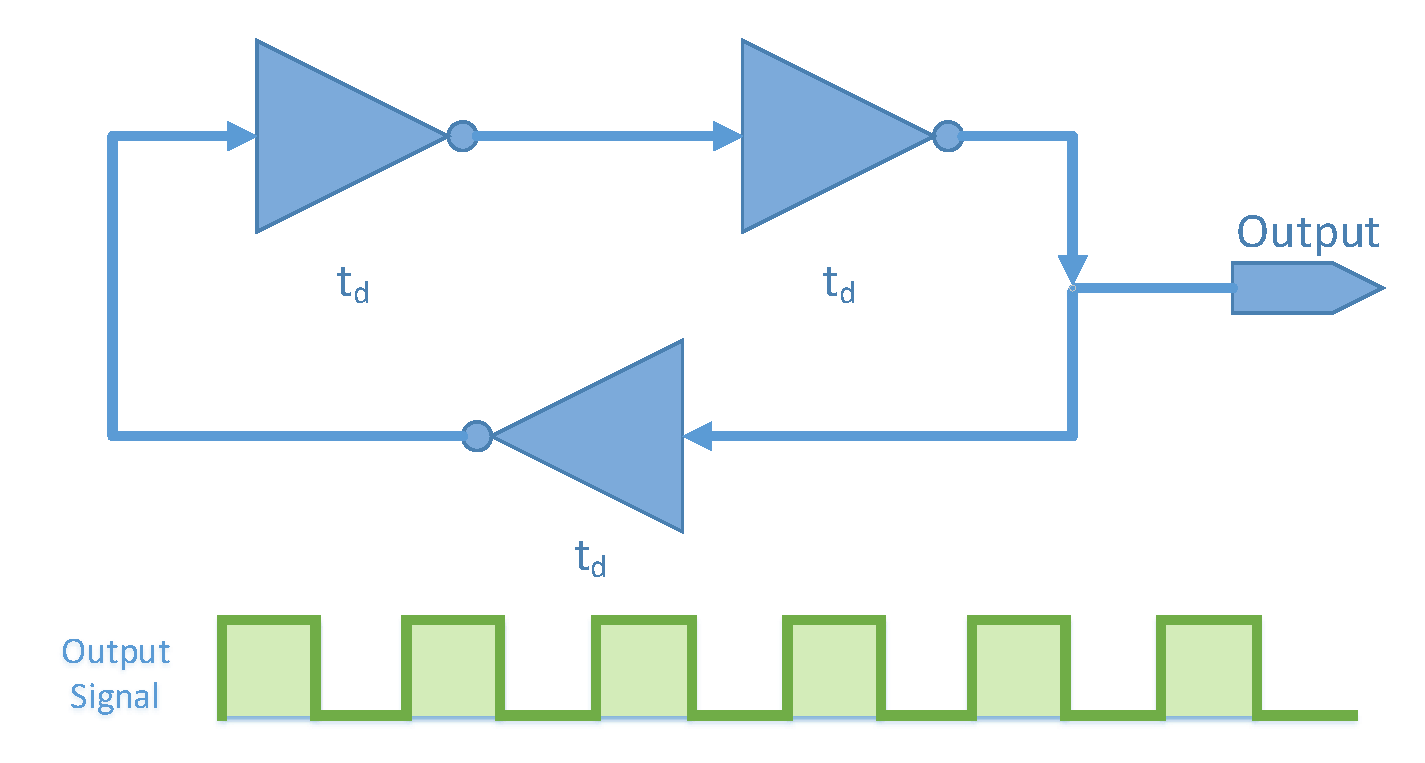
\includegraphics[width=0.5\linewidth]{./resources/ringOscillator.pdf}
      \caption{Simulation result for Listing \ref{ring-oscillator},
        output changes 15ns after the change in input.}
      \label{ring-oscillator}
    \end{figure}

  \item Using the expression from the Problem {\theproblemNumber}.3,
    write the description of a module for a 5 NOT gate ring
    oscillator. You have to design the ring oscillator such that the
    time period of the generated wave will be 30ns, assume that each
    of the NOT gate has a propagation delay of 5ns.
  \item Will a single not gate ring oscillator work? Why or why not?
  \end{enumerate}

  \hint{hint:problem-1}{Use behavioural modelling for Problem \theproblemNumber.4,
    this would allow you to assign initial state of the output and
    thus preventing the gates from entering state 'X'.}  }


\section{Data-flow Modelling}
%https://stackoverflow.com/questions/28751979/difference-between-behavioral-and-dataflow-in-verilog#28759581
Data flow modelling is a higher level of abstraction than the gate
level modelling we just studied. Describing a circuit using data-flow
modelling does not require knowledge of gates level circuit, thus it
is easier than gate-level modelling when description of large scale
circuits are written.  All the examples from Assignment 1 uses data
flow modelling.

\subsection{Continuous Assignment}
\label{continuous-assignment}
Continuous assignment in Verilog is used for data flow modelling.
These assignment starts with
\inlinev{assign} keyword. Continuous
assignment drives value into a net
(\inlinev{wire}). Following example
describes use of continuous assignment:

\pitfall{pitfall:verilog-concurrency}{Since Verilog is concurrent language unlike programming
  languages such as C,C++ or Java, all the continuous assignments are
  evaluated at the same time.}

\insertverilog{./verilog_files/continuousAssignment.v}{continuous-assignment}{Example
  usage of continuous assignment.}

Continuous assigment in Verilog can also be done implicitly, which is
assigning value on declaration of a net
(\inlinev{wire}). Implicit delcaration
of Verilog is:
\begin{lstlisting}[style=verilog-inline-style,xleftmargin=.25\textwidth]
  wire new_wire = input1 & input2;
\end{lstlisting}

\subsection{Assignment Delays}
Similar to gate-level modelling, Verilog allows specifying delays in
assignment to model real circuits. Assignment delay specify the delay
between the change of LHS and RHS of a continuous assignment. Listing
\ref{assignment-delay} shows example usage of assignment delay while
Fig. \ref{assignment-delay-sim} shows simulation result of Listing
\ref{assignment-delay}.

\insertverilog{./verilog_files/assignmentDelay.v}{assignment-delay}{Using assignment delay in Verilog.}

\begin{figure}[!h] \centering  
  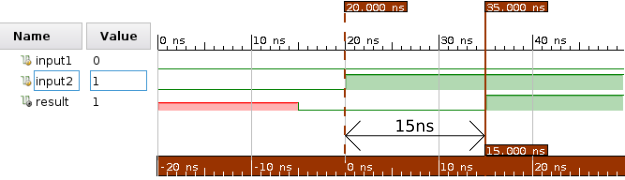
\includegraphics[width=0.8\linewidth]{./resources/assignmentDelay.png}
  \caption{Simulation result for Listing \ref{assignment-delay}, output changes 15ns after the change in input.} 
  \label{assignment-delay-sim}
\end{figure}

\insertProblem {10\%} { Multiplexer is a digital element which is used to
  select a single signal from a group of signals. Block diagram of a
  multiplexer is shown in Fig. \ref{multiplexer}, the input
  $\text{in}_1$ and $\text{in}_2$ are multiplexed and the output is
  decided using the input $\text{c}$. If the input c is 0 then
  $\text{output}=\text{in}_1$ else $\text{output}=\text{in}_2$.
  
  \begin{figure}[!h] \centering  
    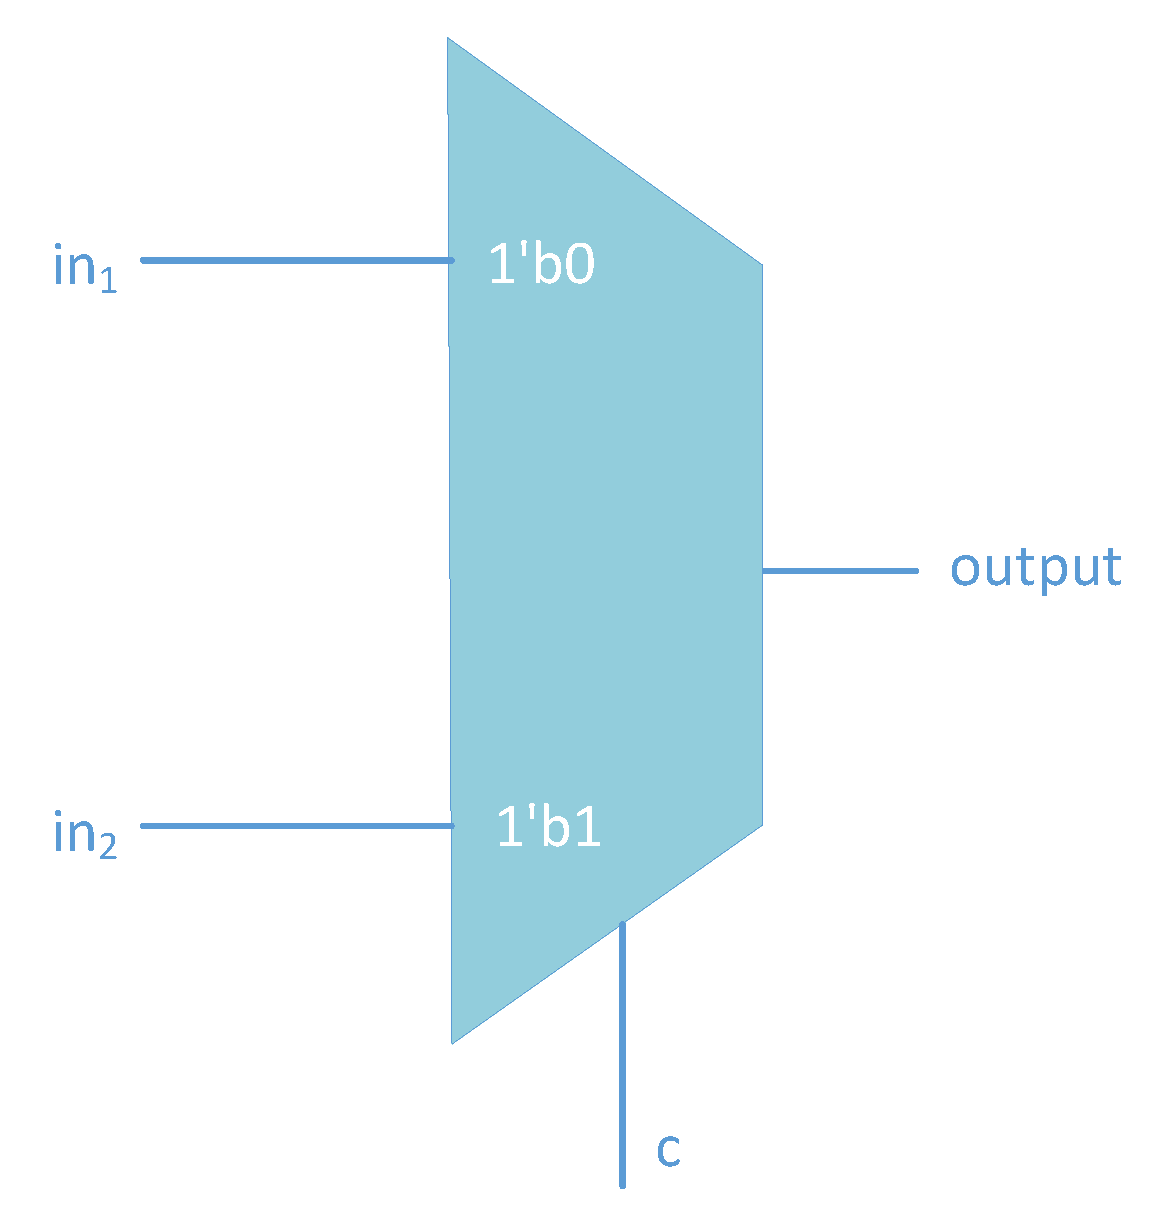
\includegraphics[width=0.3\linewidth]{./resources/multiplexer.pdf} 
    \caption{} 
    \label{multiplexer} 
  \end{figure}

  \begin{enumerate}    
  \item Write the hardware description of a 2-to-1 multiplexer using
    Verilog. You have to implement this using only data-flow
    modelling.
  \item Now suppose you want to model a multiplexer you just purchased
    from the market, which has a propagation delay of 2ns. Modify the
    module from part 1 such that the behaviour of your description
    matches the one you bought.
    
  \end{enumerate}
    \begin{table}[!ht]
      \centering
      \caption{Module attributes for problem \theproblemNumber}
      \renewcommand{\arraystretch}{1.1}
      \begin{tabularx}{0.8\textwidth}{|X|X|X|}
        \hline
        \rowcolor{greatblue}
        \color{white} Atrribute & \color{white}Name & \color{white}Size (in bits) \\
        \hline
        Module Name   & multiplexer     & \_  \\
        First Input   & in1             &  1  \\
        Second Input  & in2             &  1  \\
        Result        & result          &  1  \\
        Select Signal & select          &  1  \\
        \hline
      \end{tabularx}
    \end{table}

    \hint{hint:problem-2}{Verilog also supports the ternary operator, which has same
      behaviour as they have in programming languages.}
}
\section{Behavioral Modelling}
Behavioral modelling is an even higher level of modelling where
circuit description is written as its behaviour, this algorithmic
representation of a circuit abstracts the details of gate-level and
data flow modelling. Behavioral modelling resembles more to
programming languages such as C than it does to circuit description.


\subsection{\inlinev{reg} Element}
\inlinev{reg} element is used to represent abstract storage device in
Verilog. \inlinev{reg}s can be used to store information (single bit
or of arbitrary length using array, arrays are similar to
vectors). We'll get back to usage of \inlinev{reg} and will
differentiate it with \inlinev{wire} after studying procedural blocks.

\subsection{Procedural Blocks}
Earlier we have read about continuous assignment which allows us to
drive value to a net whenever the driver changes. This kind of
assignment allows description of only combinational circuit. To
describe sequential circuits Verilog provides procedural blocks. These
blocks are used to drive values to variables (\inlinev{reg}) only if
the condition is met.

\subsection{\inlinev{initial} Block}
\inlinev{initial} blocks in Verilog are used to specify initial values
of all the storage elements. When simulation starts simulator doesn't
know what values are to be assigned to storage elements. Initial block
begins with \inlinev{initial begin} and ends with an
\inlinev{end}. Initial blocks gets executed only once when the
simulation is started.

\pitfall{pitfall:reg-vs-wire}{Only a \inlinev{reg} can be assigned values inside an
  \inlinev{initial} block. This is because unlike \inlinev{wire} which
  are used for connection, \inlinev{reg} stores information and this
  information is unknown to the simulator at t=0. Structure of an
  initial block is given in Listing \ref{initial-structure}.}

\insertverilog{./verilog_files/initialStructure.v}{initial-structure}{Structure
  of an initial block.}

\subsection{\inlinev{always@} block}
\inlinev{always@} block in Verilog are used for describing an event
which should happen only under certain conditions, such as change in
value of one of the elements.
 
Basic structure of an \inlinev{always@} block is given in Listing
\ref{always-structure}.

\insertverilog{./verilog_files/alwaysStructure.v}{always-structure}{Structure
  of an always@ block.}

Listing \ref{always-example} shows a module which changes output only
on the positive edge of input \inlinev{clk}.

\insertverilog{./verilog_files/alwaysExample.v}{always-example}{Synchronous
  logic which changes value of result only at the positive edge of
  clk.}
 
\subsection{Blocking and Non-Blocking Assignment}
\subsubsection{Blocking Assignments}
Blocking assingments are assignments which block the simulation while
their value is being calculated. This means that the execution flow
will stop at this statement until it is executed. Blocking assignment
in Verilog is done using
\inlinev{=}. Listing
\ref{non-working-blocking-assignment} demonstrates the functioning of
blocking assignment.

\insertverilog{./verilog_files/nonWorkingSwap.v}{non-working-blocking-assignment}{Swapping bytes using blocking assignment.}  

In the above example (Listing \ref{non-working-blocking-assignment})
statement 18 doesn't gets executed until statement 17 is executed,
this is due to the use of blocking assignment.

\subsubsection{Non-blocking Assignments} 
In Listing \ref{non-working-blocking-assignment} we saw that blocking
assignments cannot be used to swap bytes, this is where non-blocking
assignments will come to use. Non-blocking assignments are evaluated
in two steps first all the RHS values are calculated at the begining
of the procedural block, and then the value is assigned to LHS when
the execution reaches particular statement.

Listing \ref{working-swap} shows how non-blocking assignments can be
used for swapping bytes.

\insertverilog{./verilog_files/workingSwap.v}{working-swap}{Swapping
  bytes using non-blocking assignment\, it works!}

\pitfall{pitfall:mixing-assignments}{It is a good HDL practice to not mix different assigments in
  a single procedural block, doing so will make your code difficult to
  read and a potential source of bugs.}

\section{Differences between \inlinev{wire} and \inlinev{reg} and where to use what}
\subsection{Legal use of \inlinev{wire}}
Wires in Verilog are used to connect two elements. They can be
assigned a value or a value can be read from them. They, however,
cannot store this value, to read something off of a wire you'll have
to drive them either with constant, other wires or regs.

\begin{itemize}
\item \inlinev{wire}s are allowed only
  in continuous assignments (page \pageref{continuous-assignment}).
\item A \inlinev{wire} cannot be
  assigned a value inside a procedural block.
\item A \inlinev{wire} can be used to
  assign a value to a \inlinev{reg} or a
  \inlinev{wire}.
\item \inlinev{wire}s can be used for I/O connections of a module instance.
\end{itemize}

\subsection{Legal use of \inlinev{reg}}
\inlinev{reg}s in Verilog are storage
elements. They, however, do not represent physical registers. Once
synthesized they can be represented by a physical register, RAM or
ROM.

 \begin{itemize}
 \item \inlinev{reg}s cannot be assigned
   a value using continuous assigment.
 \item A \inlinev{reg} can only be
   assigned a value in a procedural block.
 \item A \inlinev{reg} can be used to
   assign a value to a \inlinev{reg} or
   a \inlinev{wire}.
\end{itemize}

 \subsection{Places where both \inlinev{wire} and \inlinev{reg} are allowed}

 \begin{itemize}
 \item Both can appear on the right hand side of an
   \inlinev{assign} statement or can be
   used inside a procedural block
   (\inlinev{initial}/\inlinev{always})
   block to set value of a
   \inlinev{reg}.
 \item Can be used as inputs to a module.
\end{itemize}

 % Link to java implementation of turing machines:
 % https://introcs.cs.princeton.edu/java/52turing/

 \insertProblem {35\%} { A Turing machine is a theoretical machine which is
   used as an abstraction to real computational machines, Turing
   machine was proposed by Alan Turing in 1936. The basis of invention
   of turing machine was Alan's interest in the philosophy of
   computation. An interesting thing about the Turing machine is that
   any algorithm which is impossible to implement on Turing machine
   has never worked on any other real machine. Programming languages
   such as Java, C, C++ etc. are said to be turing complete This
   implies that anything that can be computed by a turing machine can
   be computed by these languages.

   \problemheading{Basics of Turing machine}\\ Turing machine consist
   of an infinitely long tape which has certain shapes (or characters)
   on it, this tape is traversed by a head which reads the character
   directly under it and takes appropriate movement decision. An
   example of such machine is shown in
   Fig. \ref{Fig:turing-machine-example}.

   The video at \amurl{https://www.youtube.com/watch?v=mPec64RUCsk} (9
   mins : Lecture 12 - Turing Machines (Part 1/10)) will help you
   understand the Turing machine a bit better.

  \begin{figure}[!h] \centering  
    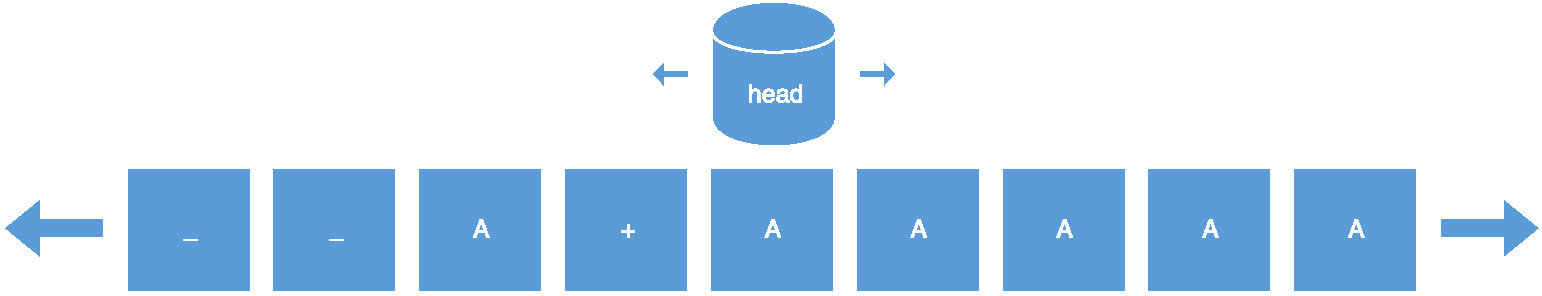
\includegraphics[width=\linewidth]{./resources/turingMachine.pdf} 
    \caption{Example of a Turing machine.} 
    \label{Fig:turing-machine-example} 
  \end{figure}

  Turing machines can be used to implement Finite state machines. To use
  a Turing machine as a finite state machine we need following
  assumptions:
  \begin{enumerate}
  \item The tape is finite in length (since it would be impossible
    to write description of an infinite tape).
  \item Each character on the tape can only be `A', `+' or `\_' where
    `A' and `+' are used for decisions while `\_' represents an unused
    tape slot.
  \item The input to the machine will be the initial configuration
    of the tape while the output of the machine will be the state of
    the tape when the machine halts.
  \item At every clock cycle the Turing machine can execute only one
    instruction.
  \item Here each possible arrangement of characters on the tape
    represents a single state in the FSM.
  \end{enumerate}

    Now consider the above mentioned Turing machine rules for a
    machine which adds up two numbers. These numbers are represented
    in base 1 (e.g. $1111_1$ to represent $4_{10}$):
    \begin{table}
      \centering
      \renewcommand{\arraystretch}{1.1}
      \begin{tabularx}{0.8\textwidth}{|X|X|X|}
        \hline
        \rowcolor{greatblue}
        \color{white} Value under head & \color{white}Direction of movement & \color{white}Write value \\
        \hline
        \vspace{0.2cm}&&\\
        A  & Right &   \\
        +  & Right & A \\
        \_ & Left &   \\
        \hline
      \end{tabularx}
    \end{table}

    Using this rule set addition of two numbers can be performed on a
    Turing machine, say for example you want to add $2_{10}$ ($AA_1$)
    and $4_{10}$ ($AAAA_1$) the trace of the Turing machine to perform
    such addition would be (Assuming the halting condition to be a
    state where head returns to the position one left to the first
    number):
    \begin{legal}
    \item \begin{textsc}\_\_[A]A+AAAA\_\_\_\end{textsc}
    \item \begin{textsc}\_\_A[A]+AAAA\_\_\_\end{textsc}
    \item \begin{textsc}\_\_AA[+]AAAA\_\_\_\end{textsc}
    \item \begin{textsc}\_\_AAA[A]AAA\_\_\_\end{textsc}
    \item \begin{textsc}\_\_AAAA[A]AA\_\_\_\end{textsc}
    \item \begin{textsc}\_\_AAAAA[A]A\_\_\_\end{textsc}
    \item \begin{textsc}\_\_AAAAAA[A]\_\_\_\end{textsc}
      
    \item \begin{textsc}\_\_AAAAA[A]\_\_\_\_\end{textsc}
    \item \begin{textsc}\_\_AAAA[A]A\_\_\_\_\end{textsc}
    \item \begin{textsc}\_\_AAA[A]AA\_\_\_\_\end{textsc}
    \item \begin{textsc}\_\_AA[A]AAA\_\_\_\_\end{textsc}
    \item \begin{textsc}\_\_A[A]AAAA\_\_\_\_\end{textsc}
    \item \begin{textsc}\_\_[A]AAAAA\_\_\_\_\end{textsc}
    \item \begin{textsc}\_[\_]AAAAAA\_\_\_\_\end{textsc} (\textbf{HALT})
    \end{legal}

    Here \textsc{[.]} represents the head of the machine.
    
    \problemheading{Questions}
    \begin{legal}
    \item Briefly describe the algorithm which would give the above
      trace (you can use psuedo code for your description of the
      algorithm).
    \item Write Verilog description for the Turing machine described
      above, use 2 bit registers to represent a single location on the
      tape. The tape of the machine will be finite in length and
      should be enough to store the above example. Your machine should
      be able to calculate this sum and return the result as 32 bit
      vector. When this result is generated the machine should also
      set the `done' output high indicating that the computation is
      completed. Please use names listed in Table
      \ref{table:problem-3-attr}. To get started you can use Hint
      \ref{hint:problem-3} and code provided in Listing
      \ref{problem-4-boiler}.
    \item Simulate the addition following two numbers using the turing
      machine you designed:
      \begin{enumerate}
      \item Your enrollment number's numerically largest digit.
      \item Your enrollment number's numerically largest digit + your
        enrollment number's least significant digit.
      \end{enumerate}
      For an example:

      If your enrollment number is $16116069$, your \textbf{Number 1}
      would be the $9$ since the largest digit would be $9$ and
      \textbf{Number 2} would be $18$ since
      $9+9=18$.

      {\color{red}NOTE:} If you fail to follow this convention your
      question will not evaluated.      
    \end{legal}
  If you want to read more interesting stuff on Turing Machines, you
  can look up for `The halting problem' on the internet.

  \hint{hint:problem-3}{ 
    \begin{enumerate}
    \item You can use a 2 bit wide vector to store the characters.
    \item Sample code to get you started with the problem is provided
      in Listing \ref{problem-4-boiler}
    \item The sample code also includes a few lines of code to
      automatically print your tape's states on every negative edge of
      the clock. To enable this you'll have to name your tape `tape',
      head's current position `current\_pos'. This is already done for 
      you in the sample code.
    \item Please note that you should use the states already defined
      in Listing \ref{problem-4-boiler} to allow the already included
      helper code to run.
    \item To calculate the `result' you can count how many `A's the 
      machine's traverses when it moves back from left to right
      beforing halting.
    \end{enumerate}
  }

  \begin{table}[!h]
    \centering
    \caption{Module attributes for problem \theproblemNumber}
    \label{table:problem-3-attr}
    \renewcommand{\arraystretch}{1.1} 
    \begin{tabularx}{0.8\textwidth}{|X|X|X|}
      \hline
      \rowcolor{greatblue}
      \color{white} Atrribute & \color{white}Name & \color{white}Size (in bits) \\
      \hline
      Module Name  & turing          & \_  \\
      Clock Input  & clk             &  1  \\
      Is Halted?   & done            &  1  \\
      Final count  & result          & 32  \\
      \hline
    \end{tabularx}
  \end{table}

  \insertverilog{./verilog_files/problem4Boiler.v}{problem-4-boiler}{Code
    to get you started with problem 4.}     
 }

 \insertProblem {35\%} {
   \begin{figure}[!h] \centering  
     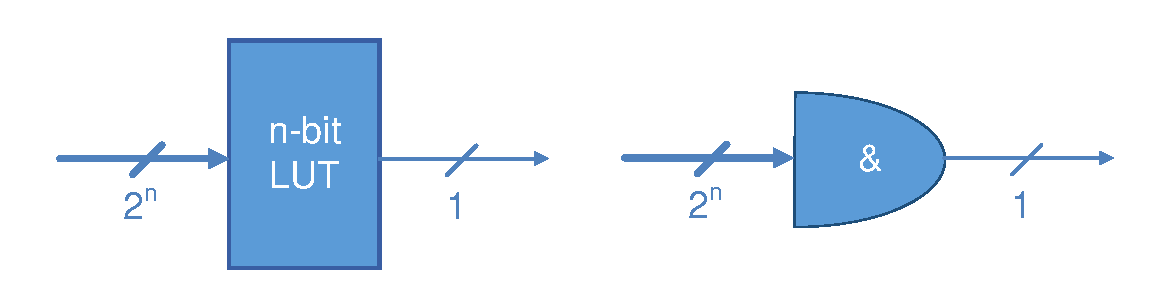
\includegraphics[width=0.8\linewidth]{./resources/and-LUT.pdf} 
     \caption{Example of an $n$-bit LUT which represents an equivalent
       $2^n$ input AND gate.}
     \label{Fig:n-bit-and-lut} 
   \end{figure}
   
   A lookup table or LUT in short is a digital structure which
   resembles a RAM, it takes an address of the location where to
   lookup an input and produces an output stored at that location. An
   LUT can be used to mimic any boolean function, an n-bit LUT table
   is one which can implement any n-bit boolean function. For example,
   a 2 bit LUT will have 4 inputs and a single bit output. Visual
   representation of an n-bit LUT is shown in Figure
   \ref{Fig:n-bit-and-lut}. Using this knowledge answer the following
   questions:

   \begin{enumerate}
     \item Design and test a 4 input AND gate using a 2 bit
       LUT. You should use names from Table
       \ref{table:problem-4.1-attr}. Take hint from the AND gate's
       truth table.
     \item Use the LUT that you designed in Problem
       \theproblemNumber.1 to implement and test a 4 input AND
       gate. You should use names from Table
       \ref{table:problem-4.2-attr}.
     \item Design appropriate modules and implement and test the
       following logic equation:
       \begin{equation}
         \text{result} = [(\text{a} \land \text{b} \land \text{c}
           \land \text{d}) \lor (\text{c} \oplus \text{a})] \odot
         (\text{d})
       \end{equation}
       For symbol reference, visit:
       \amurl{https://en.wikipedia.org/wiki/Logic_gate#Symbols}.  You
       should use names from Table \ref{table:problem-4.3-attr}.
   \end{enumerate}

   \begin{table}[!h]
     \centering
     \caption{Module attributes for problem \theproblemNumber.1}
     \label{table:problem-4.1-attr}
     \renewcommand{\arraystretch}{1.1} 
     \begin{tabularx}{0.8\textwidth}{|X|X|X|}
       \hline
       \rowcolor{greatblue}
       \color{white} Atrribute & \color{white}Name & \color{white}Size (in bits) \\
       \hline
       Module Name     & and2\_lut     & \_  \\
       Address input   & address       &  2  \\
       Lookup Result   & result        &  1  \\
       Testbench Name  & and2\_lut\_tb &  1  \\
       \hline
     \end{tabularx}
   \end{table}

   \begin{table}[!h]
     \centering
     \caption{Module attributes for problem \theproblemNumber.2}
     \label{table:problem-4.2-attr}
     \renewcommand{\arraystretch}{1.1} 
     \begin{tabularx}{0.8\textwidth}{|X|X|X|}
       \hline
       \rowcolor{greatblue}
       \color{white} Atrribute & \color{white}Name & \color{white}Size (in bits) \\
       \hline
       Module Name     & and4\_lut     & \_  \\
       Address input   & address       &  4  \\
       Lookup Result   & result        &  1  \\
       Testbench Name  & and4\_lut\_tb &  1  \\
       \hline
     \end{tabularx}
   \end{table}

   \begin{table}[!h]
     \centering
     \caption{Module attributes for problem \theproblemNumber.3}
     \label{table:problem-4.3-attr}
     \renewcommand{\arraystretch}{1.1} 
     \begin{tabularx}{0.8\textwidth}{|X|X|X|}
       \hline
       \rowcolor{greatblue}
       \color{white} Atrribute & \color{white}Name & \color{white}Size (in bits) \\
       \hline
       Module Name     & equation\_lut     & \_  \\
       Input a         & a                 &  1  \\
       Input b         & b                 &  1  \\
       Input c         & c                 &  1  \\
       Input d         & d                 &  1  \\

       Result          & result            &  1  \\
       
       Testbench Name  & equation\_lut\_tb & \_ \\
       \hline
     \end{tabularx}
   \end{table}

 }
 

 \section*{Submission Instructions}
The submissions of solutions to the assignment {\ano} should strictly
follow the following guidelines. Please read them carefully to allow
proper evaluation of the assignment.

\begin{itemize}
\item \textbf{Full screen - Screen shots} of Elaborated design, Source
  code and simulation window. Please note that only full screen
  screenshots will be considered for the evaluation. You are required
  to provide these screen shots in a PDF file with file's name being
  your enrollment
  number. \inlinev{.doc},
  \inlinev{.docx},
  \inlinev{.odt} or any other document
  format will {\color{red}not} be accepted as a substitute for the PDF
  file.

\item \textbf{Source code of each problem}: You are also required to submit
the source code file for each of the problem, if your solution to a
single problem has more than one source code files, then submit each
one of them.

\item \textbf{Single zip file submission}: Please note that the
  submission should have only a single {\color{blue}zip} file. This
  zip file would contain all the other files that you want to submit.

  \inlinev{.rar},
  \inlinev{7z},
  \inlinev{tar.gz} or any other
  archiving format will {\color{red}not} be accepted and can lead to
  disqualification of your submission.
  
\end{itemize} 

{\color{blue}For example}: If your enrollment number is 1234 and you
have created two files for solving Problem 1, while rest of the
problems have single file each:

\begin{itemize}
\item \inlinev{module_1_1.v} - Which
  contains your main module, namely
  \inlinev{module_1_1}.
\item \inlinev{andGate.v} - Which
  contains description of module andGate and is used by module
  \inlinev{module_1_1.v}
\item \inlinev{module_1_2.v}
\item \inlinev{module_1_3.v}
\item \inlinev{module_1_4.v}
\end{itemize}

Then your submission should be a \textbf{\color{blue}zip} having the
following structure:

\begin{enumerate}
\item \inlinev{1234.zip}
  \begin{enumerate}
  \item \inlinev{1234.pdf} - containing
    all the screen shots.
  \item \inlinev{module_1_1.v}
  \item \inlinev{andGate.v}
  \item \inlinev{module_1_2.v}
  \item \inlinev{module_1_3.v}
  \item \inlinev{module_1_4.v}
  \end{enumerate}
\end{enumerate}

Please note that only a single zip file will be accepted for the
submission. Using any other file format will lead to a
{\color{red}penalty}. All your files, source codes and the pdf should
be within the zip file for the submission to be considered complete.

\section*{Document History}
\begin{enumerate}
  \histitem{Sat Feb  9 14:25:45 IST 2019}{
    \begin{enumerate}
    \item Add expected module names to each problem
    \item Fix typos
    \end{enumerate}
  }
  \histitem{Mon Nov 29 15:57:13 IST 2017} {
    First Edition
  }
\end{enumerate}

\section*{Additional resources}
\begin{itemize}
  \small 
\item Stack Exchange: How are Verilog “always” statements implemented
  in hardware? \\$\rhd$ \amurl{http://bit.ly/verilogAlwaysStatement}
\item Stack Overflow: Difference between behavioral and dataflow in
  verilog \\$\rhd$ \amurl{http://bit.ly/modellingDiff}
\item Stack Overflow: How can I know if my code is synthesizable?
  [Verilog] \\$\rhd$ \amurl{http://bit.ly/synthCode}
\end{itemize} 

\section*{References}
\begin{itemize}
  \small
\item Understanding Verilog Blocking and Non-blocking Assignments
  \\$\rhd$
  \amurl{http://www.sutherland-hdl.com/papers/1996-CUG-presentation_nonblocking_assigns.pdf}
\item Verilog: always @ Blocks \\$\rhd$
  \amurl{http://inst.eecs.berkeley.edu/~cs150/fa08/Documents/Always.pdf}
\end{itemize}
\end{document}
